\documentclass[letterpaper,twocolumn,10pt]{article}
%\usepackage{times}
\usepackage{usenix,epsfig,endnotes}

%========================
%  Packages
%========================

\usepackage{graphicx,url,color}
\usepackage{amsmath}
\usepackage{amssymb}
%\usepackage{amsthm}  %<---- for a different "look" in theorems (theorem word in bold, etc.) %ACM conflict with proof definition?
%\usepackage{subfigure}
%\usepackage[tight,footnotesize]{subfigure}
\usepackage{algorithm}
\usepackage[noend]{algpseudocode}
\usepackage{times}

%\usepackage{todonotes}
%\usepackage[normalem]{ulem} %strikethrough: \sout{Hello World}
%\usepackage{lastpage} %for number of pages
%\usepackage{xspace}
%\usepackage{multirow}
%\usepackage{balance}

\usepackage[colorlinks=true,allcolors=blue,breaklinks]{hyperref}   % hyperlinks, including DOIs and URLs in bibliography
\usepackage{subcaption}
%\usepackage{caption}
\usepackage{float}

%========================
%  Macros
%========================

\newcommand{\code}[1]{\textsf{\fontsize{9}{11}\selectfont #1}}

\newcommand{\inred}[1]{{\color{red}{#1}}}
\newcommand{\remove}[1]{}
\newcommand{\Idit}[1]{[[\inred{Idit: #1}]]}
\newcommand{\eshcar}[1]{[[\inred{eshcar: #1}]]}
\newcommand{\tb}{\hspace{5mm}}

\newcommand{\sys}{Accordion}
\newcommand{\none}{NONE}
\newcommand{\basic}{BASIC}
\newcommand{\magic}{MAGIC}
\newcommand{\figw}{0.925\columnwidth}

\newcommand{\speedup}[1]{#1$\times$}
\newcommand{\tuple}[1]{\ensuremath{\langle \mbox{#1} \rangle}}

%========================
\begin{document}

\date{}

\title{\Large \bf  Playing HBase Tunes on \sys}


\author{
\remove{
Edward Bortnikov\footnotemark[1]  \tb
Anastasia Braginsky\footnotemark[1]  \tb
Eshcar Hillel\footnotemark[1] \tb 
Idit Keidar\footnotemark[1] \footnotemark[2] \\
	\footnotemark[1] Yahoo Research\ \ \footnotemark[2] Technion  \\ [2mm]
%\small Submission Type: Research	
}
Deployed-system paper
} % end author


\maketitle



%=========================================================================
%  Abstract
%=========================================================================

\subsection*{Abstract}

Distributed NoSQL data stores are now ubiquitously used for a wide range of Internet-scale applications, 
including search indexing, analytics, user data management, messaging, advertizing, online trading, and much much more.
Such data stores are commonly organized as  log-structured merge (LSM) trees, 
which replace random disk writes with sequential I/O by accumulating large batches of updates 
in an in-memory data structure. 
\remove{
and merging it with  on-disk store in the background. 
}

This paper  reports on our experience in improving the memory organization of the popular 
Apache HBase LSM-based NoSQL store. 
We present \sys, a new memory management scheme for LSM trees, which we have implemented and 
committed in HBase 2.0.
\sys\ reduces the size of the data structure holding the 
 top LSM level, namely, the dynamic memory component that absorbs writes, and utilizes the remainging 
RAM capacity to store flat static data. This  saves space and also reduces  memory management overhead (garbage collection, etc.). 
In addition, \sys\ allows for in-memory compactions (of the flat data), whereas existing LSM-based stores compact only on-disk data. 
\sys\ thus produces  fewer disk writes, which reduces disk wear as well as disk compactions. 

Perhaps surprisingly, our experiments show that memory management overhead is a more significant bottleneck than disk I/O in a
wide range of deployments and workloads, and hence \sys\ reaps more performance benefits from flattening than from in-memory compactions,
while the latter is important for extending disk lifes.

%========================

\section{Introduction} \label{sec:intro}

% NoSQL stores are popular
NoSQL key-value data stores such as Apache HBase~\cite{hbase} have become extremely popular over the last decade, 
and the range of applications for which they are used continously increases. A small sample of the recently 
published use cases includes mass-scale online analytics (Airbnb/Airstream\footnote{\small{\url{https://www.slideshare.net/HBaseCon/apache-hbase-at-airbnb}}}, 
Yahoo/Flurry\footnote{\small{\url{https://www.slideshare.net/HBaseCon/hbasecon-2015-hbase-operations-in-a-flurry}}}), e-commerce product search 
and recommendation (Alibaba~\cite{alibabahbase}), 
graph storage (Facebook/Dragon\footnote{\small{\url{https://code.facebook.com/posts/1737605303120405/dragon-a-distributed-graph-query-engine/}}}, 
Pinterest/Zen\footnote{\small{\url{https://www.slideshare.net/InfoQ/zen-pinterests-graph-storage-service}}}), etc. 

%Similarly, Imgur uses HBase to power its notifications system\footnote{\url{https://dzone.com/articles/why-imgur-dropped-mysql-in-favor-of-hbase}};
%Spotify uses HBase as base for Hadoop and machine learning
%jobs\footnote{\url{https://apachebigdata2015.sched.com}};
%web mail metadata and search serving (Yahoo Mail), 
%\footnote{\small{HBaseCon 2017 -- \url{http://hbase.apache.org/www.hbasecon.com}}}. 

% LSM trees optimize disk i/o 
The leading approach for implementation of scalable key-value storage is \emph{log-structured merge (LSM)} trees~\cite{O'Neil:1996}.
This technology is ubiquitously used by popular key-value storage libraries (e.g., LevelDB\footnote{\small{\url{https://github.com/google/leveldb}}}, 
RocksDB\footnote{\small{\url{https://rocksdb.org}}}, ScyllaDB\footnote{\small{\url{https://github.com/scylladb/scylla}}}) and distributed systems on top 
of them (e.g., Bigtable~\cite{Chang2008}, Cassandra\footnote{\small{\url{http://cassandra.apache.org/}}}, HBase, 
MongoDB\footnote{\small{\url{http://mongorocks.org/}}}, MySql\footnote{\small{\url{http://myrocks.io/}}}), etc. 
%which are employed by  Apache HBase, Bigtable, RocksDB, LevelDB, MongoDB, SQLite4, WiredTiger, Apache Cassandra,  InfluxDB, and many more.
The premise for using LSM trees is that disk access is considered the principal bottleneck in storage systems, even with today's SSD hardware~\cite{rocksdb,Tanenbaum:2014:MOS:2655363,Wu:2012:AWB:2093139.2093140}. 
The main design goal is to improve write throughput, which LSM trees do by batching writes in memory 
and periodically \emph{flushing} the memory  to disk. This way, random-access I/O is transformed to storage-friendly sequential I/O. 

An LSM tree includes a \emph{memory store} in addition to the large \emph{disk store} consisting of a collection of files. 
The memory store absorbs writes, and is periodically flushed to disk as a new immutable file. Reads search for the data
in the memory store, as well as in the disk store. The number of files has adverse impact on read performance. 
In order to reduce it, the system peridically runs a background \emph{compaction} process, which reads some files from 
the disk and merges them into a single file while removing redundant (overwritten or deleted) entries.
% For further background, see Section~\ref{sec:background}.

% Compactions hurt 
The performance of modern LSM stores is highly optimized, and yet as technology scales and real-time 
performance expectations increase, these systems face more stringent performance demands. In particular, 
they are extremely sensitive to the rate and extent of compactions. If compactions are infrequent, read performance
suffers (e.g., caching is less efficient when the data is scattered across multiple files). On the other hand, if 
compactions are too frequent, they jeopardize the performance of both writes and reads by consuming CPU 
and I/O resources. In formal terms, LSM trees struggle to balance between {\em read amplification} (the number 
of disk reads per query) and {\em write amplification} (the ratio of bytes written to disk versus bytes written to the 
database). In addition to its performance impact, write amplification accelerates device wearout, especially for SSD 
hardware~\cite{Hu:2009}. 

Enormous effort has been invested in designing compaction parameter tuning, scheduling, etc.~\cite{hbasetuning,
universalcompaction,scylladbcompaction,Sears:2012}. However, all these approaches only deal with the aftermath
of organizing the disk store as a sequence of files created upon memory store overflow events. Obviously, the more 
frequently the memory overflows, the bigger the ensuing flush and compaction toll, and the lower the overall 
system performance. Buying more memory alleviates the problem but cannot solve it completely for large datasets. 
The RAM of a typical production machine is 2-3 orders of magnitide smaller than disk space. Therefore, throughout 
its lifetime, a store is flushed to disk hundreds to thousands of times, which entails many more compactions of varying 
extents.  Our work is motivated by stretching the time between flushes without extra hardware cost, 
through better use of memory. 

% The problem
A memory store is an ordered map with {\em get} (point query), {\em scan} (range query) and {\em put} 
(point update) and {\em delete} API's. Traditionally, it is implemented as a dynamic index over a collection of data items. 
(e.g., HBase uses the standard Java concurrent skiplist\footnote{\small{\url{https://docs.oracle.com/javase/7/docs/api/java/util/concurrent/ConcurrentSkipListSet.html}}}).
The data is multi-versioned, i.e., every put creates a new immutable version of the data item it is applied to. 
This implementation suffers from two drawbacks. First, the use of a big dynamic data structure entails 
the abundance of auxiliary small objects and references, which inflate the in-memory index compared 
to its compact on-disk sibling, sorted array. The overhead is most significant when the managed objects
are small, i.e., the metadata-to-data ratio is big~\cite{Wu2015}. Second, the versioning mechanism makes 
no attempt to eliminate redundancies prior to flush, i.e., the store grows monotonically, independent in the workload. 
This is especially wasteful for heavy-tailed distributions that are prevalent in production workloads~\cite{Devineni:2015}.

% Drumroll 
We introduce \sys, an algorithm for memory store management in LSM trees. %, which addresses these problems. 
\sys\/ re-applies the classic LSM tree design principles to the memory store. Namely, it partitions this store
 into a small dynamic segment that absorbs the recent writes, and a sequence of static segments created 
 from previous dynamic segments by {\em in-memory flushes}. These segments have an optimized memory
 layout (flat index), which reduces the memory overhead. Depending on the workload, the algorithm may 
 perform {\em in-memory compactions}, which eliminate the redundant versions. Section~\ref{sec:accordion}
 fleshes out the implementation details. 
 
 In-memory flushes and compactions occur at a higher rate than their system-level siblings. They allow the system 
 flush to disk less frequently, and consequently reduce the overall I/O and the CPU cycles wasted on background maintenance
  of the LSM tree structure. In Java implementations (e.g., HBase), shrinking 
 the dynamic component results in singnificant reduction of GC overhead. Furthermore, since the static indices 
 are flat, the system can place them in off-JVM heap memory, thereby exploiting more RAM. Finally, reducing the 
 disk I/O decelerates the hardware wearout period. 

% Status
\sys\/ is implemented in HBase production code; it is generally available starting the HBase 2.0 release. 
The extensive evaluation process led to \sys's adoption as default memory store implementation. 

% Experiments
In Section~\ref{sec:eval} we experiment with \sys\ implementation in HBase in a range of scenarios.
We study production-size datasets and data layouts, as well as multiple storage types (SSD and HDD). 
We conclude that the algorithm's contribution to the overall system performance is substantial, 
especially when working with small objects and heavy-tailed (Zipf) distributions. For example, \sys\/ 
improves the system write throughput by up to $40\%$, and reduces the tail read latency by up to 
\inred{XX\%}. In parallel, it reduces the write amplification by up to \inred{XX\%}. Surprisingly, we see 
that in most settings, disk I/O is \emph{not} the principal bottleneck. Rather, the memory management 
overhead is more substantial: the improvements are highly correlated with GC reduction. 

\sys\/ got its name for periodically growing and shrinking the system's memory footprint, similarly 
to accordion bellows. As our experiments show, this movement delivers fresh air, reduces congestion, 
and improves the end-to-end system performance. 


 

\section{Background}\label{sec:bg}
%\input{bg}

\section{\sys} \label{sec:accordion}

We describe  \sys's architecture and basic operation in Section~\ref{ssec:overview}.
We then discuss in-memory compaction policies  in  Section~\ref{ssec:policies}
and implementation details in Section~\ref{ssec:impl-details}. 

\subsection{Overview} \label{ssec:overview}

\begin{figure}[tbh]
\center
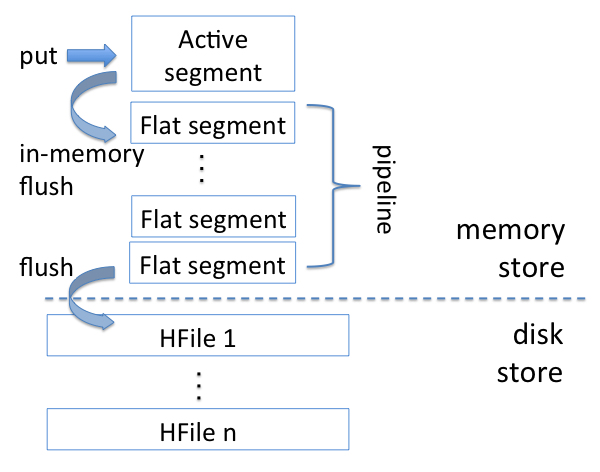
\includegraphics[width=\columnwidth]{Accordion} 
\caption{\sys's compacting memory store architecture adds a pipeline of flat segments between the active segment and the snapshot. 
The memory store includes a small dynamic active segment 
and a pipeline of flat segments. A disk flush creates a snapshot of the pipeline for writing to disk.}
\label{fig:accordion}
\end{figure}

\sys\ introduces a \emph{compacting} memory store to the LSM tree design framework. In contrast to the traditional memory store, 
which maintains RAM-resident data in a single monolithic data structure, \sys\ manages data as a \emph{pipeline} of 
\emph{segments} ordered by creation time. At all times, the most recent segment, called \emph{active}, is mutable;
it absorbs  put operations. The rest of the segments are immutable. Get and scan operations retrieve data from all  segments, 
 similarly to a traditional LSM tree read from multiple files. 
 
 Figure~\ref{fig:accordion} illustrates the \sys\ architecture. It is parameterized by two values:
\begin{itemize}
\item  $A$ -- the fraction of the memory store allocated to the active segment; and 
\item $S$ -- the upper bound on the number of immutable segments in the pipeline. 
\end{itemize}

\noindent
As our experiments show (Section~\ref{sec:eval}), the most effective parameter values are quite small, 
e.g., $0.02 \leq A \leq 0.05$, and $1 \leq S \leq 5$.

The memory store dynamics are as follows. 
Once the active segment grows to its size bound (a fraction $A$ of the memory store's size bound), an \emph{in-memory flush} is invoked.
The in-memory flush makes the active segment immutable and creates a new active segment to replace it. 
The replaced active segment is then added to the pipeline in one of three ways. 
\begin{description}
\item[Flattening of intra-segment search indices.] 
In case there is available space in the pipeline (the number of pipeline segments is smaller than $S$), 
the segment is simply flattened. This involves replacing dynamic segment indices such as skiplists by 
compact ordered arrays, which are suitable for immutable data. 
\end{description}
Flattening reduces the MemStore's memory footprint, which delays  disk flushes, positively affecting both read latency  (by increasing the MemStore's hit rate) and write volume.

Once the number of immutable segments exceeds $S$, \emph{in-memory compaction} applies one of the following mechanisms: 
\begin{description}
\item[Merging pipeline segments' search indices.]
 \remove{ % Off-heap stuff omitted due to lack of evaluation
 % To Do: move to conclusions
  An additional advantage of the flat layout  is that in managed environments, 
 the index can be relocated to off-heap (unmanaged) memory, which can improves performance predictability 
 through reduced garbage collection jitter~\cite{alibabahbase}. 
}
This process replaces multiple segments with one by creating a single index covering data that resides 
in the original segments. This is a lightweight process that does not eliminate redundant 
data versions.
%, and hence does not involve physical data copy. 
\item[Merging pipeline segments' data.]
This process extends the above with redundant data elimination -- it 
creates a flat index with no redundancies, and disposes redundant data cells. 
\remove{ % Slab stuff omitted due to lack of evaluation
In case the memstore manages its cell data storage internally, the surviving cells are relocated
to new slabs; otherwise, the redundant cells are simply de-referenced, and later garbage-collected.    
}
\end{description} 
The choice of compaction mechanisms to employ is guided by the policies described in Section~\ref{ssec:policies} below.

Flushes to disk work the same way as in a standard LSM tree. A disk flush shifts all pipeline segments to the snapshot. The pipeline is emptied and ready to absorb new flat segments. The snapshot's immutable flat segments are not part of the pipeline, and are freed once they are written to storage. The background flush process merges the snapshot
segments while eliminating  redundancies, and streams the result to a new file. 

In case the disk flush process empties the pipeline while an in-memory compaction process is attempting to merge some segments, the latter aborts.  This behavior is valid since in-memory compaction is an optimization.

\subsection{Compaction Policies} \label{ssec:policies}

There is a tradeoff between the two in-memory compaction mechanisms. Merging only search indices without removing redundancies is a lighter-weight process.  Moreover, this approach is friendly to the managed memory system because the entire segment is freed at once, whereas 
the data-merging alternative burdens the memory management system (in particular, the garbage collector) by
constantly releasing small objects. On the other hand, the index-merging approach  
consumes memory for overwritten data; this is significant in production-like heavy-tailed distributions where some keys are frequently overwritten.
By removing these redundancies, the data-merging approach further delays disk flushes, which both improves read latency  (thanks to more 
queries being satisfied from memory) and reduces write volume.

In our HBase deployment, we implemented two policies corresponding to these two in-memory compaction approaches:
\begin{description}
\item[\basic] (low-overhead). Once a segment becomes immutable, flatten its index. Once the pipeline size exceeds $S$, 
merge all segment indices into one.  
\item[\eager] (high-overhead, high-reward under self-similar workloads). 
Once a segment becomes immutable, merge its index and data with the current (single) pipeline segment.
% In addition to \basic\/ mechanisms, eliminate data redundancies across pipeline segments.
\end{description}

Our experiments (reported in the next section) show that the \eager\ policy is typically too aggressive, in particular when $A$ is small,
and the benefits from reducing the memory footprint are offset by the increased management (and in particular, garbage collection) overhead.
We therefore present in this paper a third policy:
\begin{description}
\item[\adp] (the best of all worlds)\footnote{\small{Not committed to production code yet.}}. A heuristic that chooses 
whether to apply data compaction (as in \eager) or not (as in \basic) based on the level of redundancy in the data 
and the perceived cost-effectiveness of compaction. \adp\ works at the level of a single LSM store, i.e., triggers 
redundancy elimination only for those stores where positive impact is expected. 
\end{description}

\adp\ uses two parameters to determine whether to perform redundancy elimination.
The first is a throttling parameter $t$ based on the amount of data that can benefit from redundancy elimination. 
Initially, $t=0.5$; it then grows exponentially by $2\%$ with the number of in-memory flushes, and is reset back to 
the default value (namely $0.5$) upon disk flush. Thus, $t$ is bigger when there is more data in the MemStore.
The second parameter, $u$, estimates the ratio of unique keys in the memory store based on the 
fraction of unique keys encountered during the previous merge of segment indices. 

Note that the accuracy of $u$ at a given point in time depends on the number of merges that occurred since the last disk flush
or data-merge.
Initially, $u$ is zero, and so the first in-memory compaction does not employ data-merge.
Then, the estimate is based on the $S$ merged components, which at the time for the second in-memory compaction
is roughly one half of the relevant data, since the pipeline holds $S-1$ unmerged components. 
Over time, $u$ becomes more accurate while $t$ grows. 

\adp\/ triggers redundancy elimination with probability $t$ if the fraction of redundant keys $1-u$ exceeds a parameter 
threshold $R$. The rationale for doing so is that prediction based on $u$ becomes more accurate with time, whence 
compactions become more important because the component is bigger and more space can be saved.


\remove{
\begin{description}
\item[\emph{Unique ratio}] $u$ -- an estimate of the fraction of unique keys out of the total number of items in the segment. 
This value is estimated by counting duplicates encountered during merge, which does not induce extra overhead since
merged items are compared in any case. The \emph{unique\_ratio}  is an under-estimate of the actual redundancy because it does not 
take into consideration duplicates that were already present during flattening. Nevertheless, since the active component
is typically quite small, the error due to the under-estimate is significant only when the component is still small 
(has not undergone many merges), and compaction is therefore less important.
\item[\emph{success\_probability}] -- an estimate of the probability of a compaction yielding the expected benefits based on recent history.
Here, we define an expected space reduction threshold below which compaction is not cost-effective. 
We initialize the \emph{success\_probability} to some default value (e.g., $0.5$). 
Then, if compaction yields the expected benefit (i.e., frees up more space than the threshold) we increase the \emph{success\_probability},
and otherwise decrease it. The \emph{success\_probability} is reset to its default value upon flushes. 
The rationale for using \emph{success\_probability} is that its prediction becomes more accurate with time, whence 
compactions become more important because the component is bigger and more space can be saved.
\end{description}
}

\subsection{Implementation Details} \label{ssec:impl-details}

A compacting memstore is comprised of an active segment and a double-ended queue (pipeline) of inactive segments. 
The pipeline is accessed by read APIs (get and scan), as well as by background disk flushes and in-memory compactions. 
The latter two modify the pipeline by adding/removing/replacing segments. These modifications happen infrequently. 

The pipeline readers and writers coordinate through a lightweight copy-on-write, as follows. The pipeline object is versioned. 
Each modification promotes the version number, and atomically swaps the global reference to the new version clone. Note
that cloning is inexpensive -- only the segment references are copied since the segments themselves are immutable. 

The reads access the segments lock-free, through the version obtained at the beginning of the operation. If a disk flush
is scheduled in the middle of a read, a segment may migrate from the pipeline to the pre-flush snapshot buffer. The correctness of
reads  is guaranteed by scanning the pipeline clone first. This way, a segment may be encountered twice but no data is 
lost. The scan algorithm filters out the duplicates. 

In-memory compaction is a read-modify-write operation, which swaps one or more segments in the pipeline 
with a new segment built from their data. This operation's atomicity is guaranteed by compare-and-swap (CAS), 
which flips pipeline version only if the latter did not change since the compaction started.  For example, in-memory
compaction fails if a disk flush concurrently removes some segments from the pipeline.
% (Section~\ref{ssec:overview}). 

 

\section{Deployment in HBase} \label{sec:hbase}

\section{Empirical study} \label{sec:eval}
We compare the performance of 4 memory management strategies 
\begin{description}
\setlength{\itemsep}{0pt}
  \setlength{\parskip}{0pt}
\item[\none] -- which does no compaction of the data, this was previously the default in HBase.
\item[\basic] -- which compacts the representation of the index; this is the default in HBase 2.0.
\item[\eager] -- which compacts both the data and index.
\item[\magic] -- which compacts the index or both the data and the index based on the workload.
\end{description}

We compare the strategies by measuring their throughput and latency. In addition we measure the write volume, that is the number of KB written to the file system, and the cumulative gc time of each run.

The results of the following experiments are presented:
(1) demonstrating the insight from different sets of experiments showing that gc overhead is a great throughput predictor,
(2) write-only workload - comparing all 4 strategies,
(3) mixed read-write workload - showing reduction in read latencies of \basic\ and \magic\ strategies with respect to \none.
(4) evaluating different settings of the \basic\ strategy in order to find its optimal configuration,

\paragraph{Experiment setup.}

Our experiments run on 2 clusters with different hardware. 
The first cluster consists of five 12-core Intel Xeon 5 machines with 48GB RAM and 3TB 
SSD storage, interconnected by 1G Ethernet. 
The second cluster consists of five 8-core 
Intel Xeon E5620 servers with 24GB RAM and 1TB magnetic drive. The interconnects  are 1Gbps Ethernet. 
We denote these clusters as the SSD cluster and HDD cluster, respectively.
In both clusters we allocate three nodes to HBase nodes, 1 master and 2 region servers, one to simulate the client whose performance we measure, and one to simulate background traffic
as explained below. Each HBase node runs both an HBase region server or master and the underlying 
Hadoop File System (HDFS) server.
 
A region server runs within 8GB JVM container, with G1GC memory management. We use default configuration which allocates 40\% of the heap to memstore (roughly 3GB) and 40\% of the heap to block cache. 
Number of number of flush threads is set to 10, and  the limit on number of store files before blocking is set to 25.

The traffic is driven by a client running the popular YCSB benchmark~\cite{Cooper}. 
We run write-only and mixed read-write workload where keys are chosen from either a zipfian or a uniform distribution over a data set of 100 millions items.
In all the experiments we create a table with 4 columns (in a single column family) which is pre-split into 50 regions. 
Each update operation writes 25 Bytes values to all 4 columns of a single key, namely writing 100 Bytes of data. To increase the load updates are batched at the client side; buffer size is 10KB
Each read operation reads a single column of a single key (a cell).


\paragraph{GC overhead.}

Our experiments show that in write-only workloads gc and throughput have a very high correlation. 
Figure~\ref{fig:gc-throughput-log2} plots the scatter graph of cumulative gc time vs write throughput of several write-only experiments with varying settings in different strategies. It clearly shows that  the lower the gc overhead is, the higher the throughput is.
Specifically, there is a negative linear correlation between their values on a log-log scale.

\begin{figure}[htb]
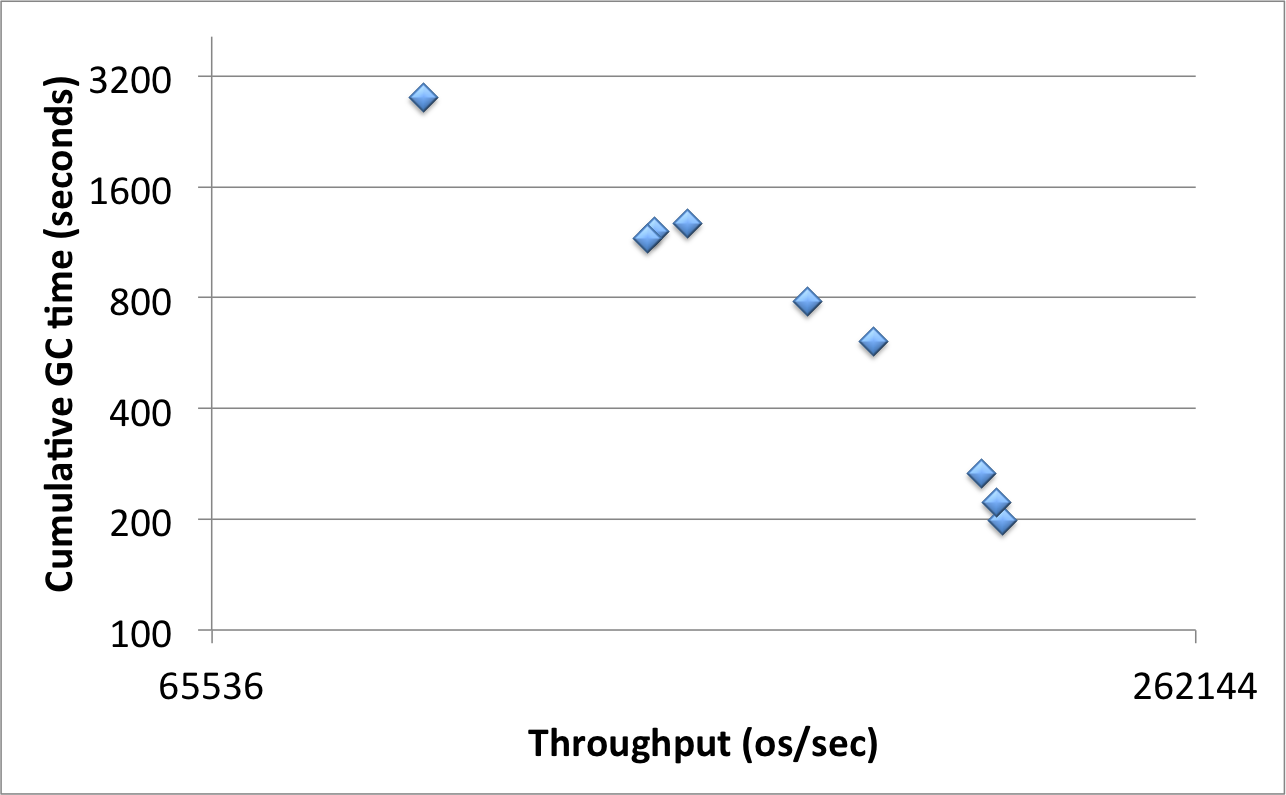
\includegraphics[width=\figw]{Figs/gc-throughput-log2.png}
\caption{{\bf GC-Throughput correlation.} Log-log scale plot of the cumulative gc time vs write throughput in different settings shows negative linear correlation.
}
\label{fig:gc-throughput-log2}
\end{figure}


\paragraph{Write-only workload.}
Each run creates an empty 50 regions table and then utilizes 12 threads to run 500 million update operations, each writing to all columns. Each such run is repeated 5 times. 
We measure total  throughput and total volume of MB written to files. We present here the performance results of the run with the median throughput among 5 runs.

Figures~\ref{fig:throughput-ssd} and~\ref{fig:throughput-hdd} depict the lift in throughput \basic, \magic, and \eager\ achieve over \none in ssd and hdd, respectively.
Tables~\ref{fig:counters:ssd} and ~\ref{fig:counters:hdd} present the number of flushes, disk compactions and WAL files generated during the experiment.
Figures~\ref{fig:volume-ssd} and~\ref{fig:volume-hdd} depict the write volume in every setting. 
\magic demonstrates the tradeoff between throughput and write volume. As we increase the compaction threshold more in-memory compaction are triggered which degrades the throughput but at the same time reduces the write volume.
At the extremes are \basic\ with the highest throughput and \eager with lowest write volume.
\basic\ and \magic\ both run with $2\%$ active segment. In SSD the limit on the size of the pipeline is 5 and in HDD it is 4.
\eager\ runs with $25\%$ active segments and limit of 2 on the size of the pipeline.
The uniques thresholds for \magic\ are $0.2$, $0.35$, and $0.5$.



\begin{figure}[htb]
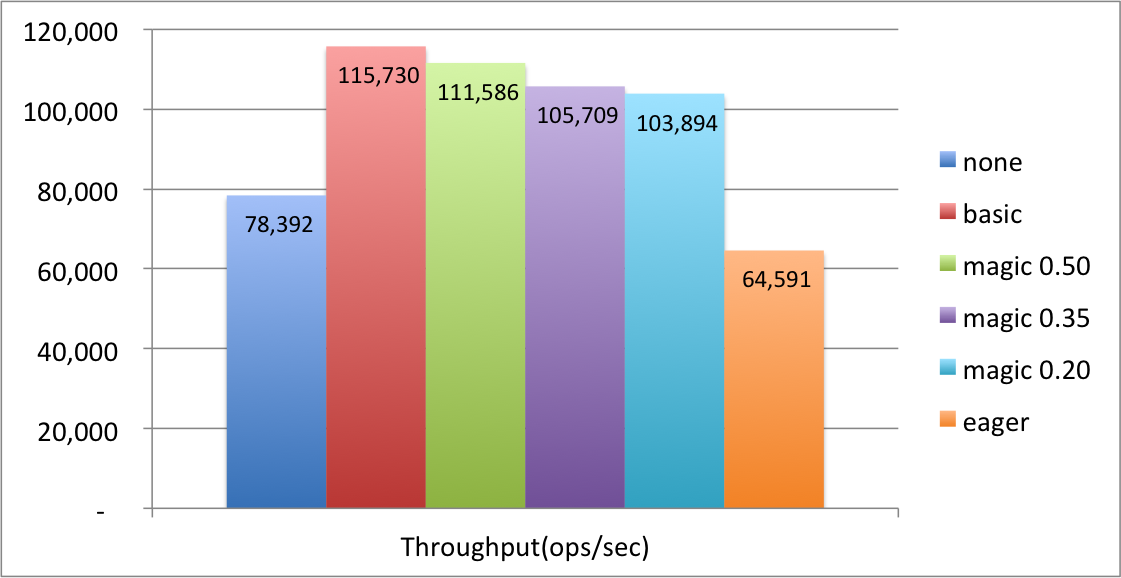
\includegraphics[width=\figw]{Figs/throughput-ssd.png}
\caption{{\bf  Throughput measured in SSD.} Zipfian distribution.
}
\label{fig:throughput-ssd}
\end{figure}

\begin{figure}[htb]
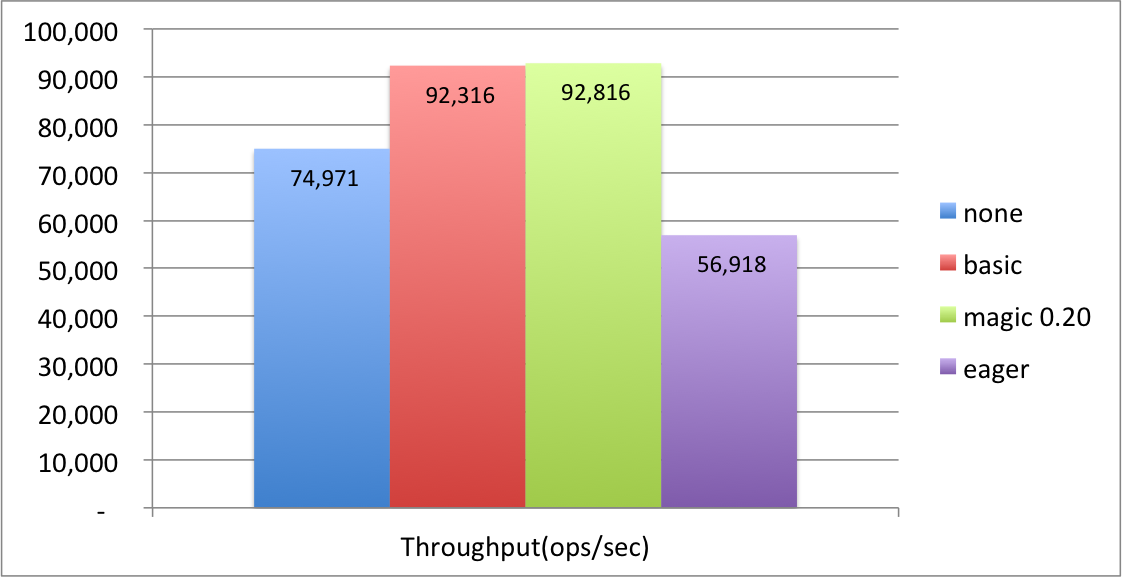
\includegraphics[width=\figw]{Figs/throughput-hdd.png}
\caption{{\bf  Throughput measured in HDD.} Zipfian distribution. 
}
\label{fig:throughput-hdd}
\end{figure}


\begin{figure}[!t]
  \centering
  
  \begin{subfigure}[tb]{\columnwidth}
      \centering\small
    \begin{tabular}{|c|c|c|c|}
      \hline
      Strategy & $\#$flushes & $\#$compactions & $\#$WAL files\\
      %\hline
      \hline
      \none & 1468	&524&	789 \\
\basic & 1224&	355&	806 \\
\magic\ 0.50 &922&	309&	678 \\
\magic\ 0.35 & 754&	261&	615 \\
\magic\ 0.20 & 631	&209	&533 \\
\eager\ & 695	&242&	490 \\
      \hline
    \end{tabular}
	\caption[]{SSD}
    \label{fig:counters:ssd}
  \end{subfigure}
  
  \begin{subfigure}[t]{\columnwidth}
    \centering\small
    \begin{tabular}{|c|c|c|c|c|}
      \hline
        Strategy & $\#$flushes & $\#$compactions & $\#$WAL files\\
      %\hline
      \hline
      \none & 1504 & 548 & 743 \\
\basic & 1210 & 443 & 808 \\
\magic\ 0.50 & 879 & 316 & 695 \\
\magic\ 0.35 & 711 & 248 & 650 \\
\magic\ 0.20 & 630 & 216 & 556 \\
\eager\ & 667 & 242 & 536 \\
      \hline
    \end{tabular}
	\caption[]{HDD}
    \label{fig:counters:hdd}
  \end{subfigure}


  \caption{Number of flushes, disk compactions, and WAL files created in different settings}
  \label{fig:counters}
\end{figure}


\begin{figure}[htb]
%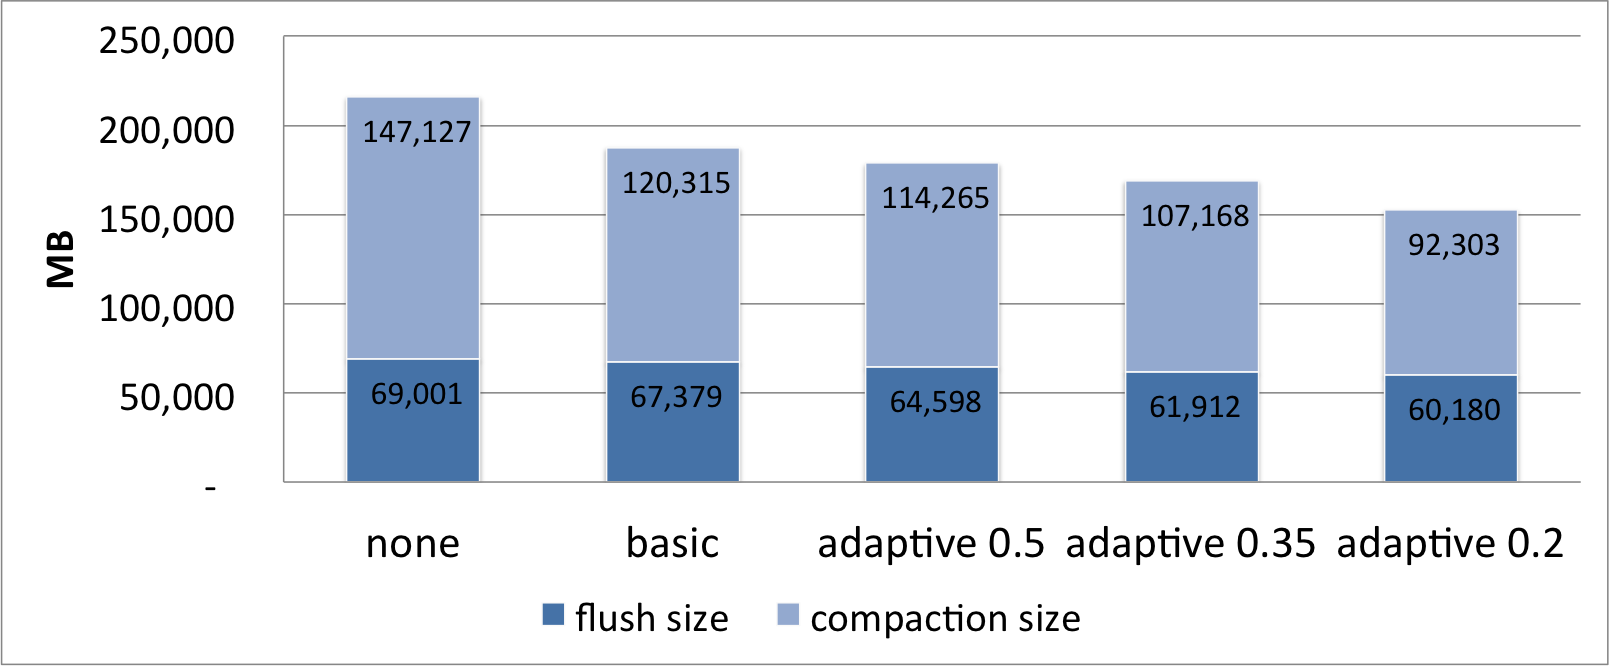
\includegraphics[width=\figw]{Figs/volume-ssd.png}
\caption{{\bf  Write volume in SSD.} Zipfian distribution.
}
\label{fig:volume-ssd}
\end{figure}

\begin{figure}[htb]
%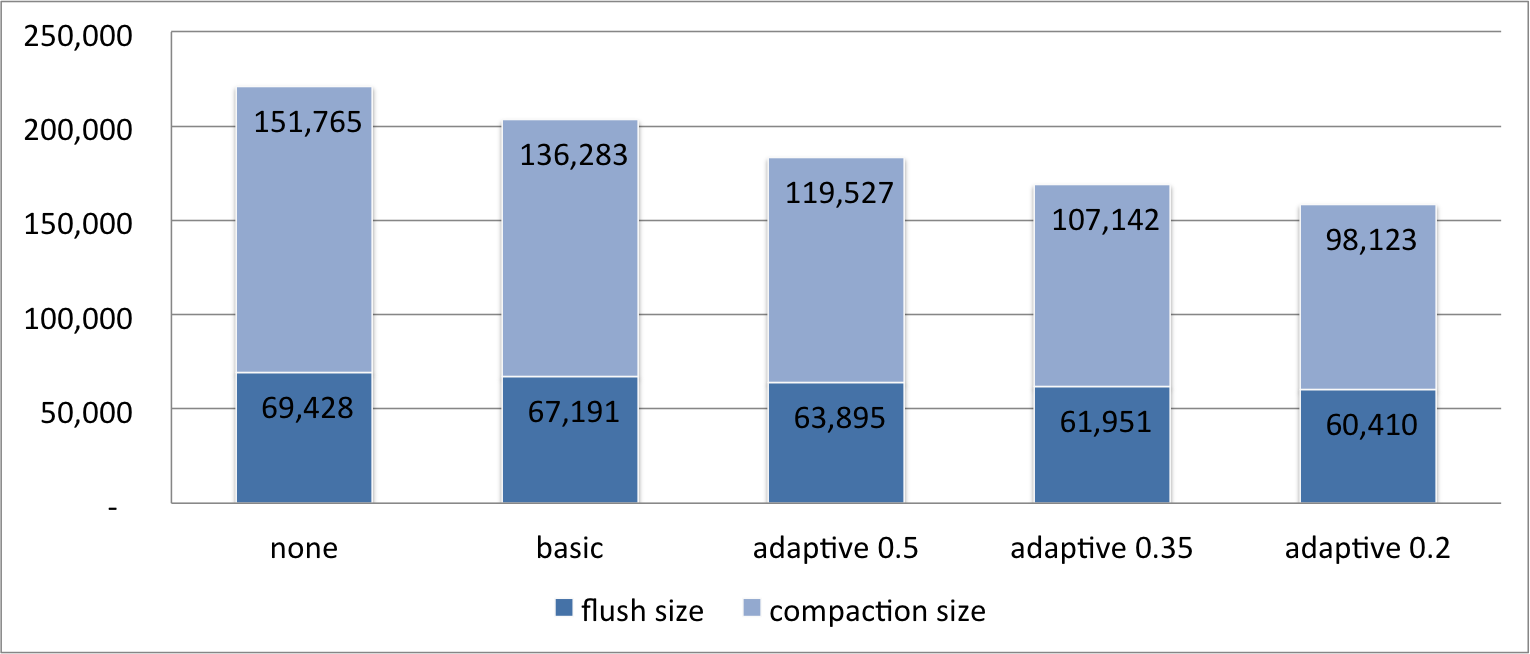
\includegraphics[width=\figw]{Figs/volume-hdd.png}
\caption{{\bf  Write volume in HDD.} Zipfian distribution.
}
\label{fig:volume-hdd}
\end{figure}




\paragraph{Mixed workload.}
Each run is comprised of two phases. 
The first phase creates an empty 50 regions table. It then loads the table with 10GB of data by running 100 million update operations chosen uniformly at random, each writing to all columns. 
The second phase measures the performance of a single thread running 150,000 read operation. 
We measure the 50-th, 75-th, 90-th, 95-th and 99-th percentiles.
An additional YCSB client is used to run background traffic. 
This client utilizes 12 threads to run update operations while we measure the read operations. 
Both reads and background traffic are chosen from a zipfian distribution.
Each such run is repeated 3 times. 

Figure~\ref{fig:latency-speedup-hdd} depicts the latency speed-up \basic\ and \magic\ achieve over \none.

\begin{figure}[htb]
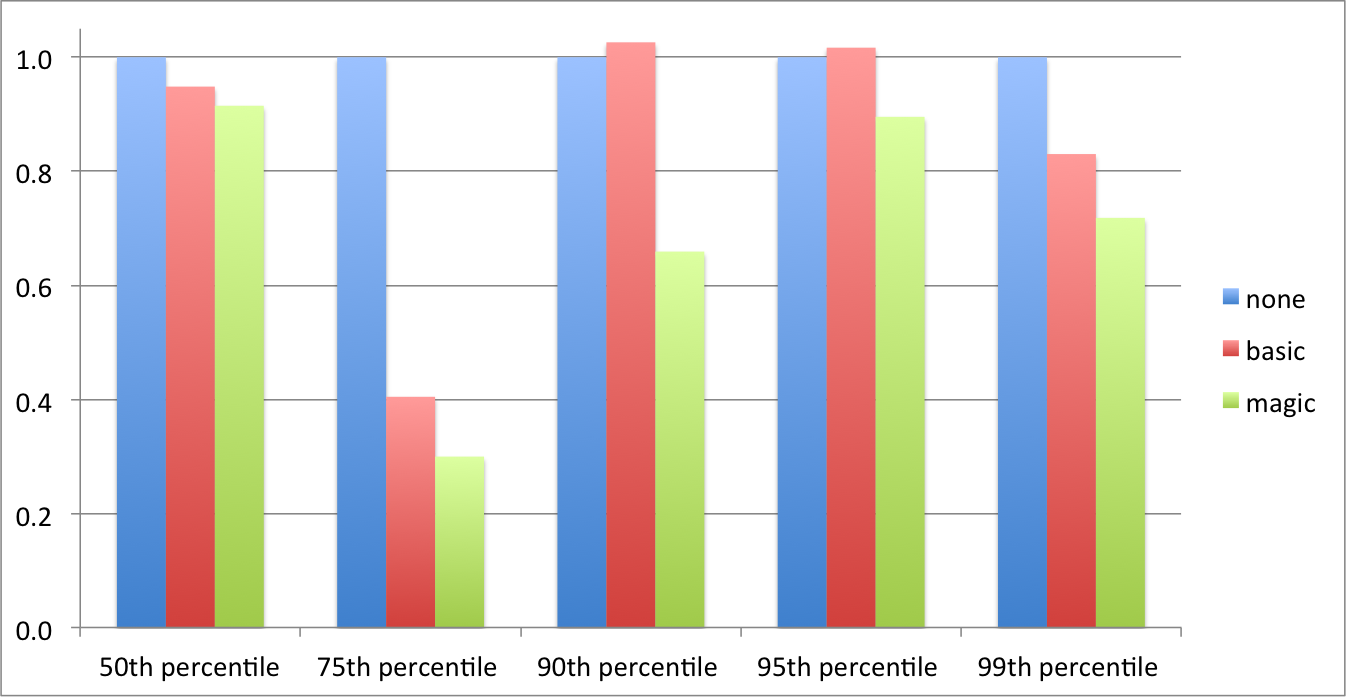
\includegraphics[width=\figw]{Figs/latency-speedup-hdd.png}
\caption{{\bf Latency speed-up in HDD.} 
}
\label{fig:latency-speedup-hdd}
\end{figure}

\paragraph{Parameter exploration.}
One of the main sources for memory management overhead is the skip-list data structure used to index the dynamic fraction of the memory component.
Not only it is bigger in size compared to a flat index it is also fragmented whereas static index is stored in a consecutive block of memory, therefore it incurs smaller overhead in terms of allocation, gc and cache misses.
We evaluate \basic\ strategy with different dynamic fraction sizes. We measure their throughput in write-only workload with zipfian distribution.
The throughput results of all runs are depicted in  Figure~\ref{fig:dynamic-fraction}. 
The \none\ strategy has no static portion in the memory component therefore its throughput is added at the point where the dynamic fraction size is equal to 1.0.
Figure~\ref{fig:dynamic-fraction} shows that indeed the store scales as the dynamic fraction size decreases. 

\begin{figure}[htb]
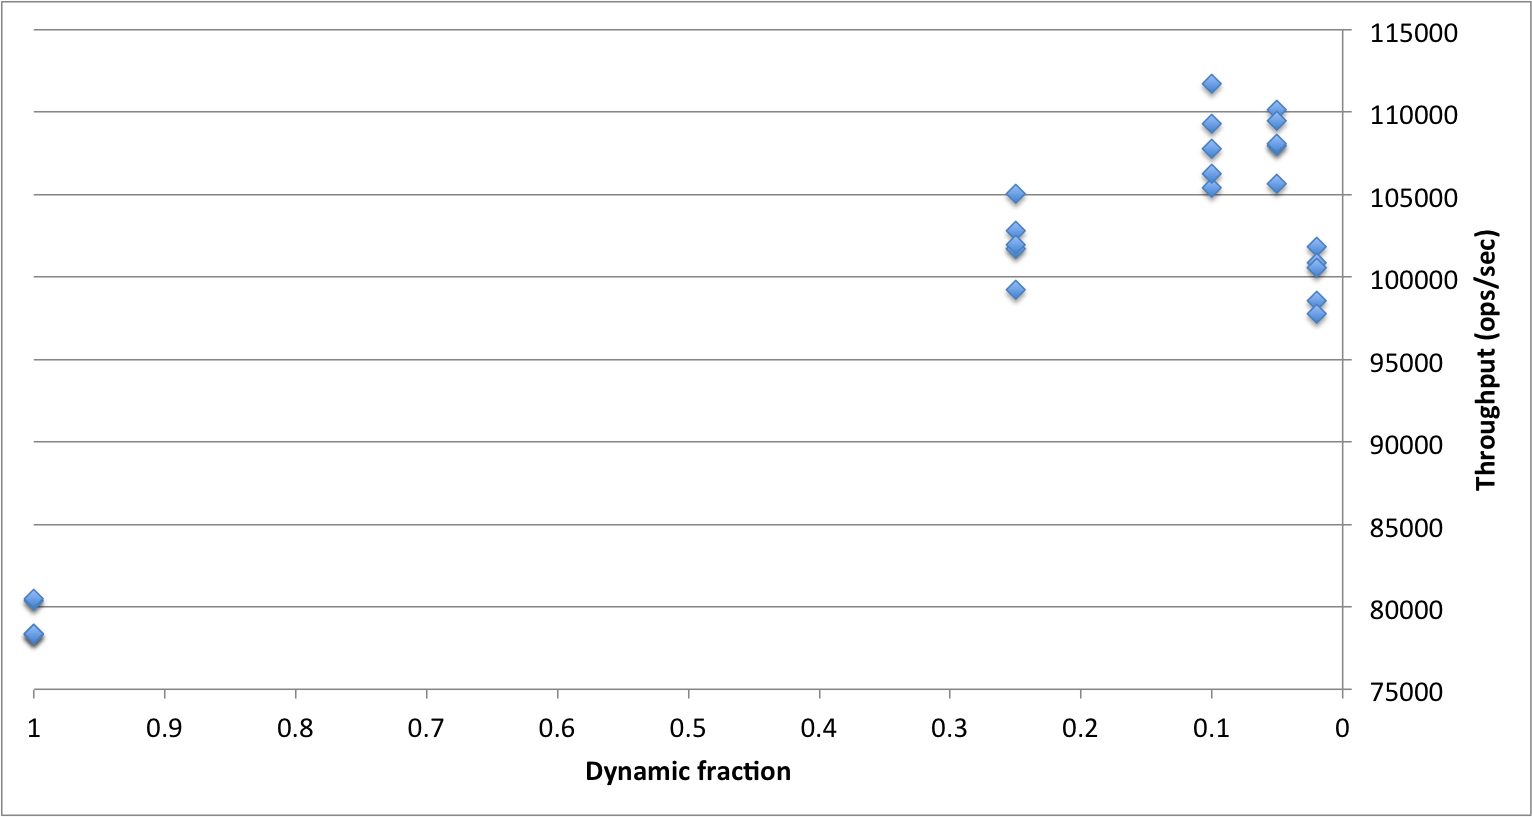
\includegraphics[width=\figw]{Figs/dynamic-fraction-1.png}
\caption{{\bf Dynamic fraction tuning.} The throughput increases as the dynamic fraction size decreases.
}
\label{fig:dynamic-fraction}
\end{figure}

When the dynamic fraction is less than $10\%$ it is clear that merging it into the much bigger static data over and over again can be inefficient as it creates a new index and dismisses the old one. 
The alternative is to enable several segments to wait in the pipeline before they are merged to a single segment. This helps with creating new index less frequently.
On the flip side, each segment in the pipeline calls for a separate scanner during read operations which can degrade their performance.
%Hence, we run the same experiments as explained above, varying the limit for the size of pipeline.
Figures~\ref{fig:pipeline-1-ssd} and~\ref{fig:pipeline-1-hdd} depict the throughput results as a function of the pipeline size. Peak throughput is with XX entries in the pipeline.

\begin{figure}[htb]
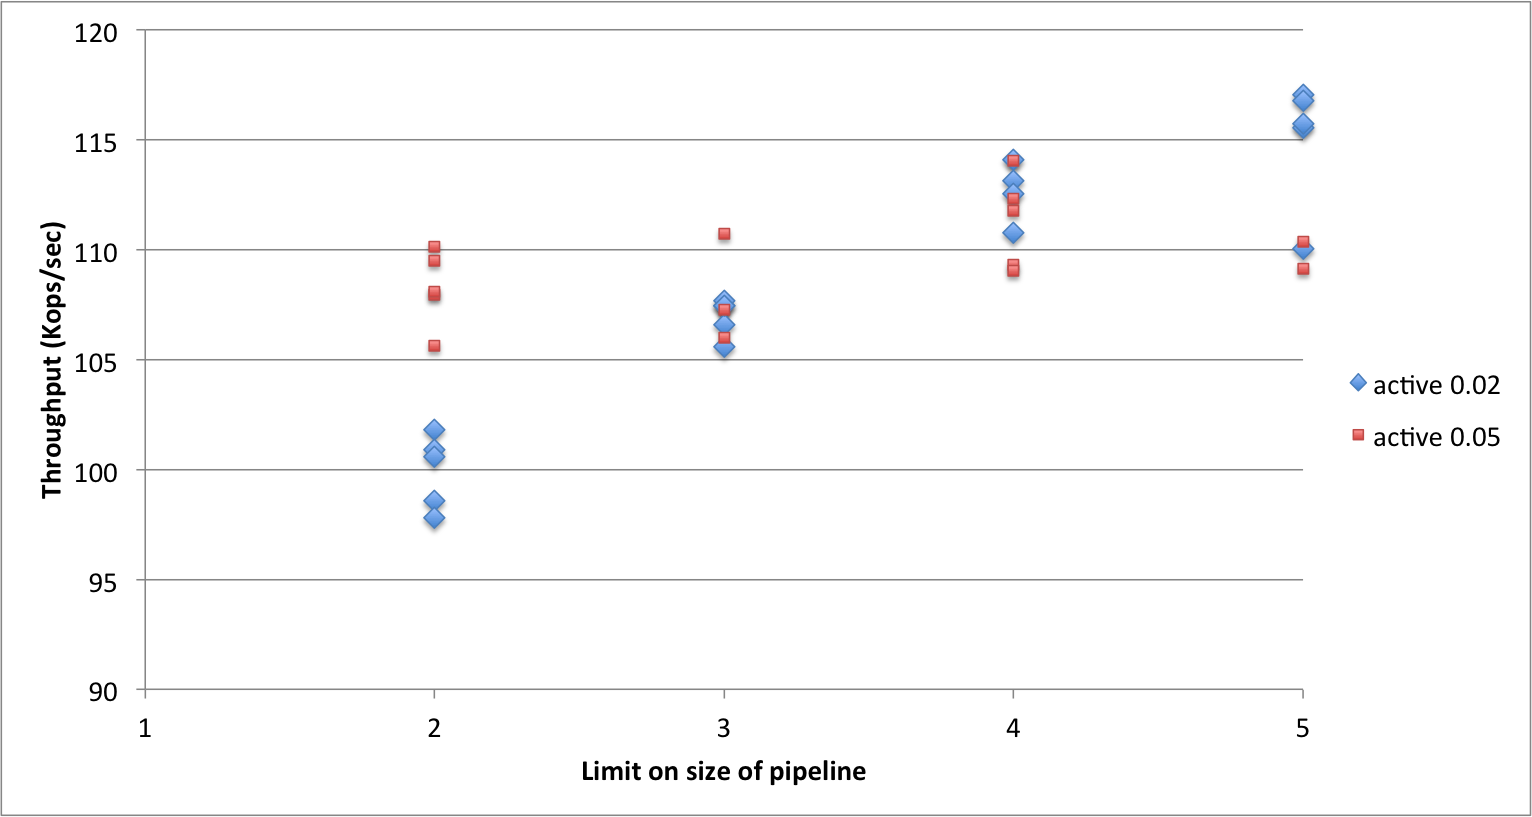
\includegraphics[width=\figw]{Figs/pipeline-1-ssd.png}
\caption{{\bf Pipeline size tuning - SSD.} 
}
\label{fig:pipeline-1-ssd}
\end{figure}

\begin{figure}[htb]
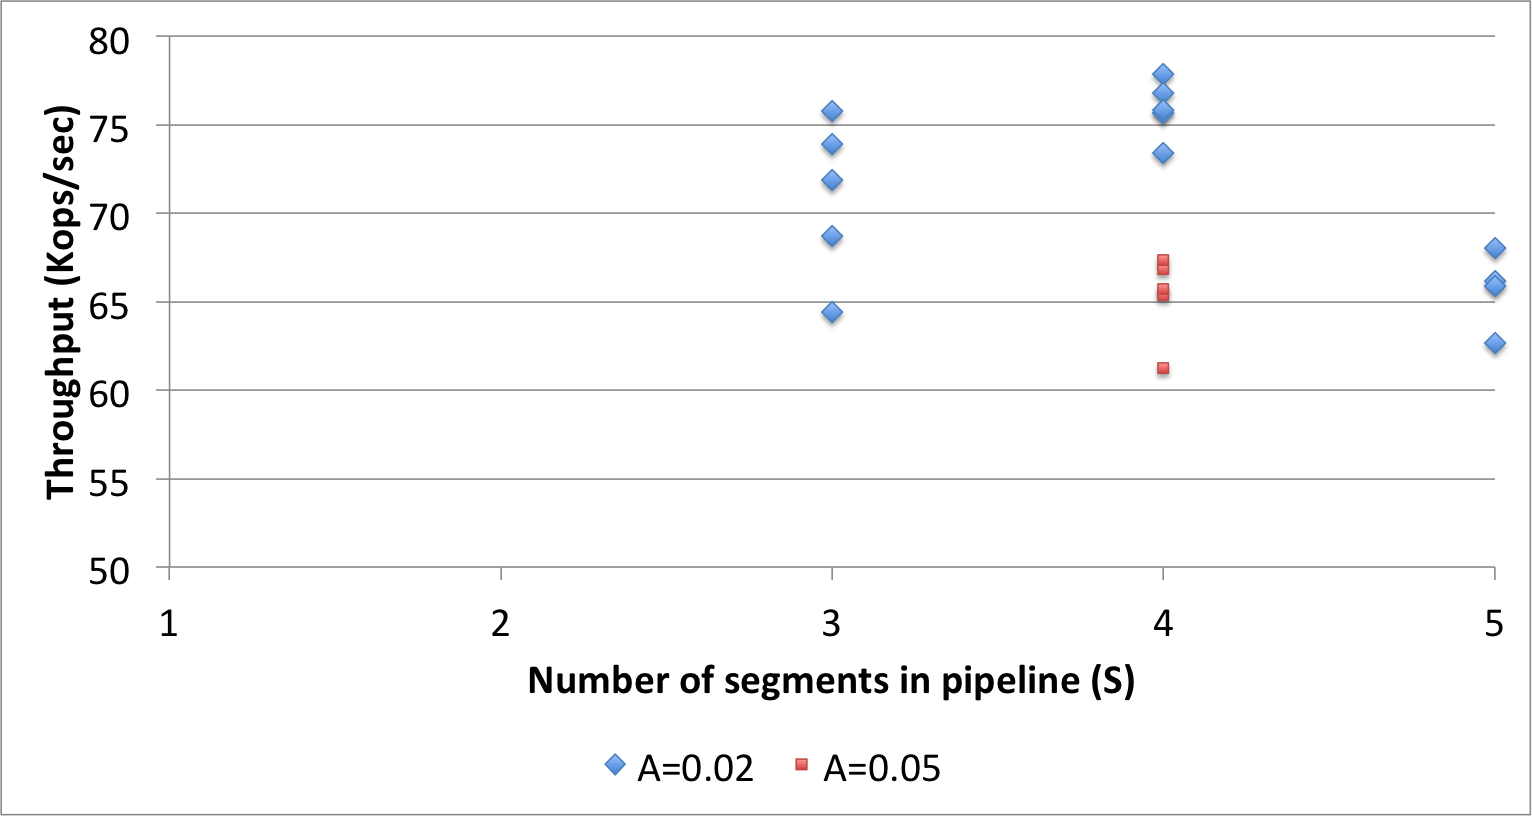
\includegraphics[width=\figw]{Figs/pipeline-1-hdd.png}
\caption{{\bf Pipeline size tuning - HDD.} 
}
\label{fig:pipeline-1-hdd}
\end{figure}

With a different experimental setup the tuning results are different.
For example when running similar workload with 100 regions and 16GB heap per region server we get different results.
\begin{figure}[htb]
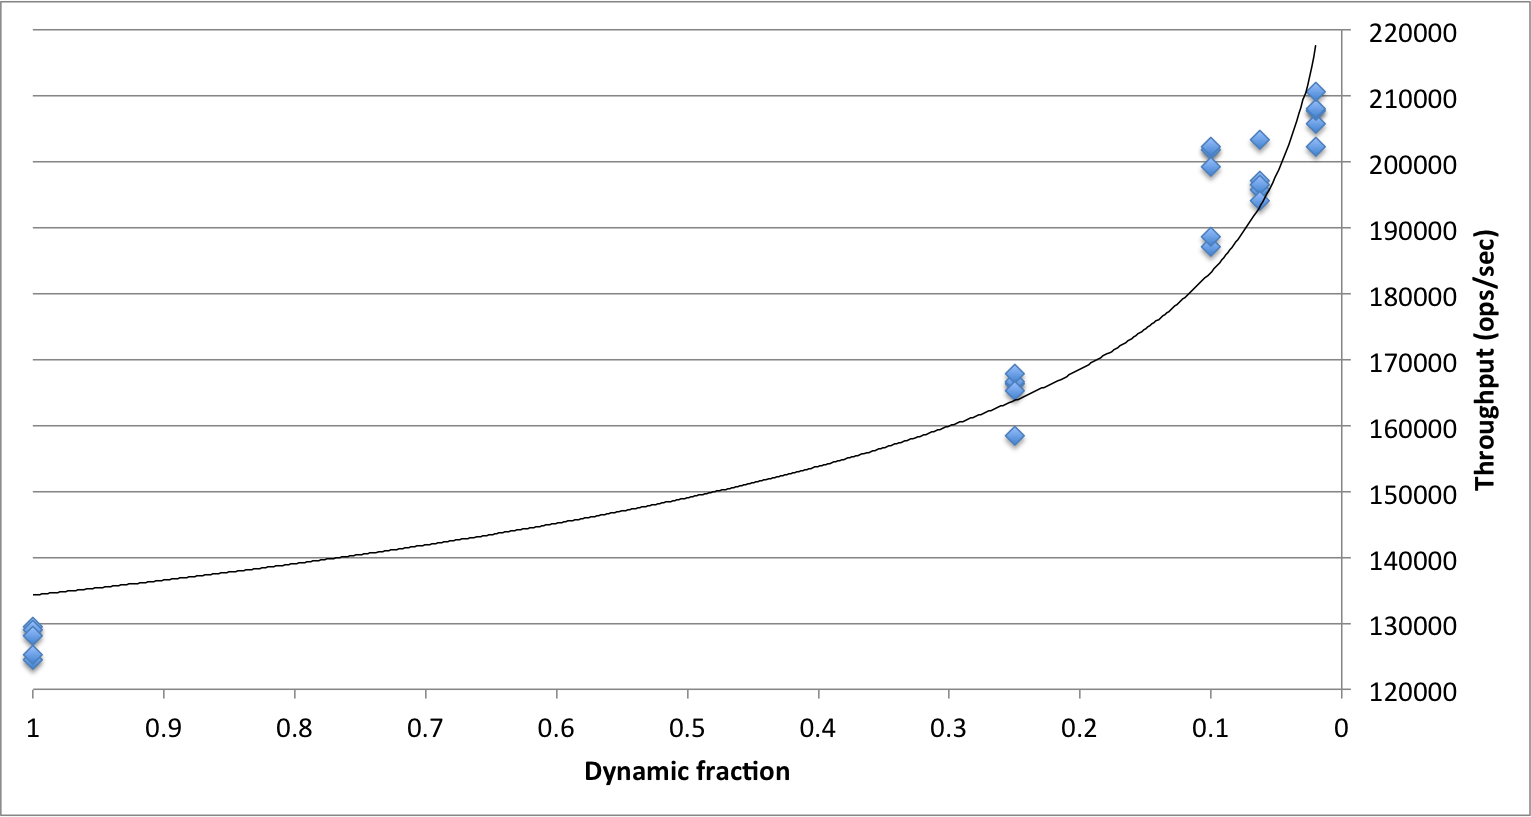
\includegraphics[width=\figw]{Figs/dynamic-fraction-2.png}
\caption{{\bf Dynamic fraction tuning.} 
}
\label{fig:dynamic-fraction-2}
\end{figure}

\begin{figure}[htb]
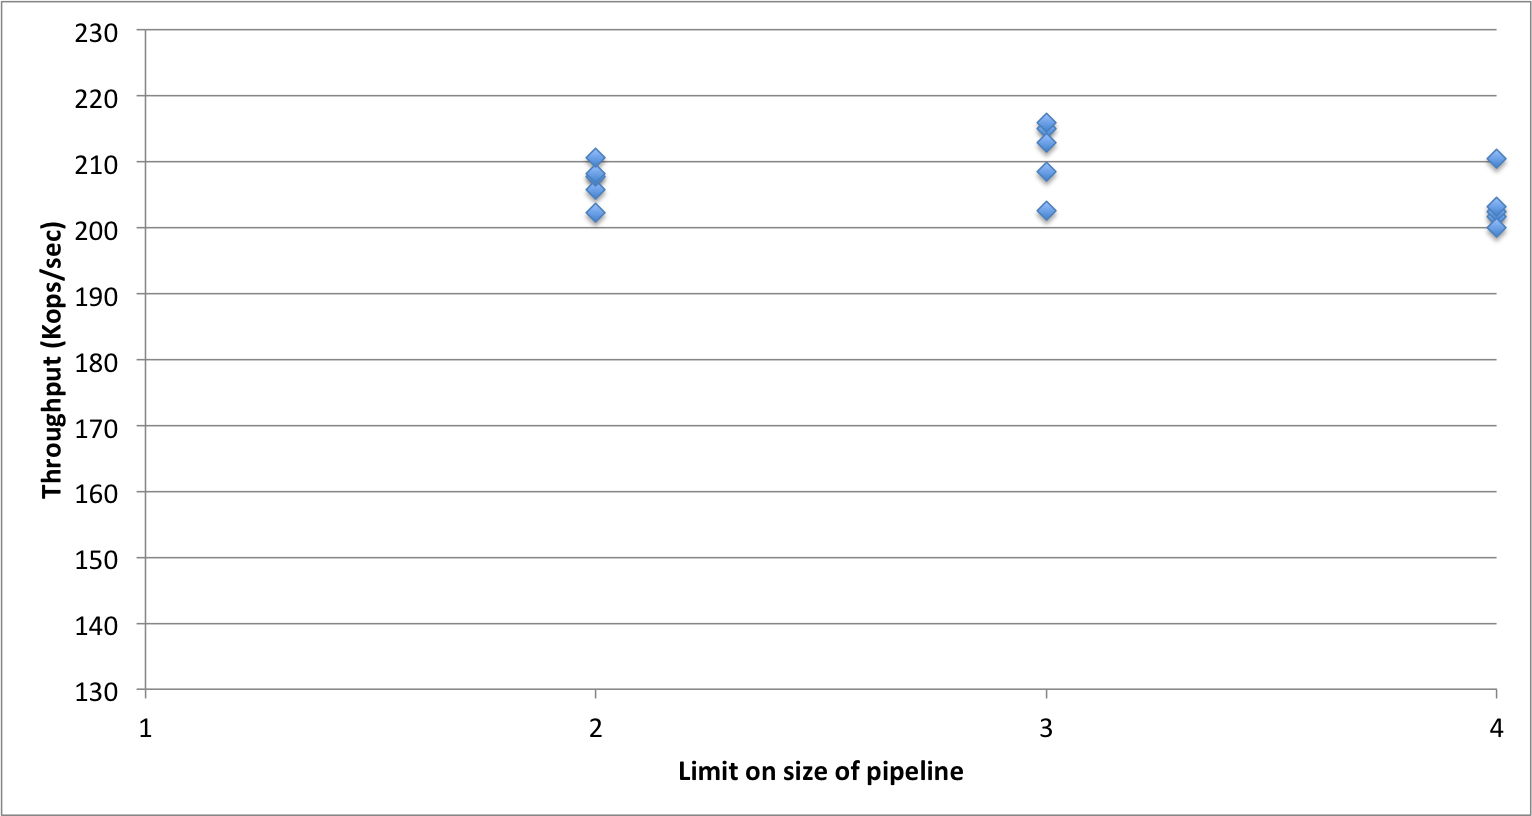
\includegraphics[width=\figw]{Figs/pipeline-2.png}
\caption{{\bf Pipeline size tuning.} 
}
\label{fig:pipeline-2}
\end{figure}



\section{Conclusion} \label{sec:conclusions}


%\subsection*{Acknowledgments}

\newpage

\bibliographystyle{acm}

\bibliography{refs}

\end{document}
